% Every document has to start with a documentclass declaration
\documentclass[11pt]{article}

% Everything after documentclass and before "\begin{document}" is called the preamble. 
% This is where you put in optional packages to control the look of the paper
\usepackage{amsmath} % necessary for most math symbols
\usepackage{setspace} % allows double or one-half spacing
\usepackage{lscape} % allow landscape pages for tables
\usepackage[top=1.25in,bottom=1.25in,left=1in,right=1in]{geometry} % adjust margins
\usepackage{graphicx} % figure management
\usepackage{epstopdf} % converts eps figures to pdf
\usepackage{booktabs} % expanded table options
\usepackage{dcolumn} % align decimals in tables
\usepackage{natbib} % bibliography commands
\usepackage{tabularx} % auto-size table columns
\usepackage[T1]{fontenc} % this ensures that special characters write to PDF properly

% In the preamble you also put in meta-data that can be used on the title page
\title{A Title for Your Paper\thanks{Contact information. I am not a huge fan of the asterisk next to the title, but it isn't obvious where this should go. You could alternatively use one of the authors - preferably the corresponding author.}} 
\author{ % enter author names, with affiliation
    Dietrich Vollrath \\ 
    University of Houston
    \and
    Zippy Zperson \\
    University of Houston
}

\date{\today}

\begin{document}
\maketitle
\thispagestyle{empty}

\begin{abstract} % We'll be adding an abstract to your title page with this 
\noindent This is a style guide for Latex papers for use by graduate students at the University of Houston. Notice that this is \textbf{not} centered on the page. Having it centered with make it look ragged. It should be flush left. I have also put in a no-indent command, so that the abstract does not indent. This gives the abstract a nice block look. The title page should have an empty page style, so that no page number appears. Put the keywords and JEL codes inside the abstract environment so they are sized appropriately and are flush with the abstract.\\

\noindent \textbf{Keywords:} separated by commas, words or short phrases \\

\noindent \textbf{JEL classification:} O1, M1, or other JEL codes
\end{abstract}

\newpage % This tells TeX to start a new page, not surprisingly
\setcounter{page}{1} % This will reset the page number to 1

\section{Introduction}
\onehalfspacing Here you begin with your interesting description of your paper. I have set the line spacing to one-half, which is preferred. The baseline font size here is 12 points. I prefer to use 11 point, as 12 point makes the text look very large, but this is not a severe issue.

For equations, including specifications for regressions, Latex will automatically number every equation. Ideally, you should only allow numbering for equations that are subsequently referenced later in the paper. For example, we should have
\begin{equation}
    Y = X^2 \label{EQ_ref}
\end{equation}
and another equation
\begin{equation}
    Z = W + X. \nonumber
\end{equation}
Now, since I refer to equation (\ref{EQ_ref}) here in the text, it has a number. And each time an equation is referenced, it should be inside parentheses. In constrast, the second equation should not have a number, because it isn't explicitly referenced in the text.

Speaking of references, both tables and figures should be referred to using capital letters, as in Table \ref{ivtable_B} or Figure \ref{FIG_dens_rurd}. 

\section{Figures}
There are entire books written about how to design informative figures. I cannot possibly give you enough information here to ensure every one that you produce is perfect. Figures are very much a trial and error process. But I do have a few pointers. Many of these refer to specific questions or problems with Stata figures.

\begin{enumerate}
    \item Do not use a background color. For example, default Stata figures have that awful blue color. Remove it with "graphregion(color(white))" as an option. The figure will blend into the page.
    \item Make sure the y-axis labels can be read left/right (not up/down). 
    \item Any numbers in the axes should have a digit before the decimal. For example, 0.1 versus .1
    \item There are ways to format figures to use a font similar to Latex (Times New Roman is the default). 
    \item Use smaller symbols and thinner lines than are the defaults
    \item Don't over-decorate the figure with borders, lines, etc. The example in Figure \ref{FIG_dens_rurd} is nice because it is simple.
\end{enumerate}

\section{Tables}
You should use the ``booktabs'' package, and the options available, to format your tables. There are a series of rules you should observe in tables.

\begin{enumerate}
    \item Never use vertical lines. If you feel that you need a vertical line to separate the left hand side of a table from the right, then you need to create a \textit{new} table.
    \item Never use doubled horizontal lines. Single horizontal lines are sufficient, and with the booktabs package, you can create appropriate ones that span several columns, or the entire table. 
    \item Numbers for columns (e.g. ``(1)'') should be the last row of the header to the table, followed by a midrule. Above the column numbers you can label columns with information about their specifics.
    \item The table number and caption should appear above the table. Do not use bold or italics in the caption. 
    \item The notes after the table should be introduced with ``Notes:'', and you may use bold or italics to highlight this. The notes should be flush left, not centered. The notes should be set at ``footnotesize''. Things to include in the notes:
        \begin{enumerate}
            \item Say standard errors are included in parentheses.
            \item Method of calculating standard errors. 
            \item The meaning of the significance stars if you use them.
            \item Control variables included in each regression in the table, if they are not shown explicitly
            \item A reference to the specification equation in the text, if available.
            \item If there is an excluded category for a categorical variable in the table, list it.
            \item Whatever else may be necessary for someone to understand what is going on. 
        \end{enumerate}
    \item The key distinction between regresions (i.e. different samples, different estimation method, different data, etc.) should be listed in the header, not in the notes.
    \item Never (ever!) use the raw variable name from Stata or other software to label the rows or columns of your table. Put in readable names.
    \item Always precede a decimal with a digit, as in 0.1
    \item Rescale your regressions or results so that you report no more than 3 decimal places. 0.00000027 is not legible to a reader.
    \item Align the decimal point within a column if is necessary to compare coefficients within a column. It is not always necessary if your main purpose will be to compare coefficients across columns.
    \item Space the columns equally. This can be done easily with the tabularx package, or manually in your specification of the table.
    \item Standard errors are preferred to a t-statistic. Use parentheses around them.
    \item If you must put in ``significance stars'', place them next to the coefficient. Use *** for 1\%, ** for 5\%, and * for 10\%. Do not get cute or innovative with the symbols. People are used to seeing the asterisks.
    \item Strive to have your paper fit on a single page, and it should not overlap that standard margins or the page number at the bottom. You can use the ``small'' or ``footnotesize'' font adjustments to fit the table. There are no good reasons to have tables that span multiple pages.
    \item For a regression table, if you are not going to mention or talk about a specific coefficient, it is fine to not show the actual estimates. Put in a row at the bottom indicating the control was included, or list the controls included in the table notes.
    \item If you use rows at the bottom of the table to indicate ``Yes/No'' for inclusion of things like fixed effects, then there should be some variance across columns in the answer to ``Yes/No''. If all the columns include something, then that should be listed in the table notes, not the table itself. 
\end{enumerate}

Note that making these formatting choices makes it hard to write out the full table command directly from Stata (or other packages). It is often useful to format the header and footer of the table in your paper, and input only the cells of the table. 

Table \ref{TAB_beta_crops} shows another example of a table formatted according to many of these rules. It is a little heavy on the use of lines to denote sub-samples, but it means that you can interpret what the difference is between columns without having to read the text, for the most part. This isn't perfect, if you haven't read the paper at all, then this won't perfect sense. But given a cursory read of the paper, you'd be able to see the point quickly. The table uses input files from Stata for the numbers, so you never have to retype or copy/paste. The unimportant control variables are not shown, because they are not important to the discussion.

The tables are all on separate pages, at the end of the paper. Use the clearpage command in Latex, and the ``[!htb]'' code at the beginning of the table code to ensure each table shows up at the top of the new page. Putting tables at the end seems inconvenient. It is now the norm for working papers. One issue is that you cannot ensure that the tables will show up in the right place in the text, making it even harder to find where they are.

\section{Citations}
In text, you should use author/date citations, as opposed to using numbers or keys. People do not want to flip back to the bibliography to see who you are talking about. 

There are some journals and sub-fields (economic history is one example) where the bibliography entry for a citation is presented immediately in a footnote following the use of the citation. That is not the standard, though, and all of your bibliography entries should appear in a separate reference section immediately following the main text of the paper.

Here's an example of citing \citet{barro2016} and then \citet{ajs2016}. Here's an example of a parenthetical citation \citep{barro2016}, and then a parenthetical citation involving multiple papers \citep{barro2016,ajs2016}. Note that in parenthetical citations, you do not use a second set of parentheses to denote the year. You use a comma, and separate different papers with a semi-colon. 

In terms of the bibliography, there are an almost infinite number of styles to adopt. APA, Chicago, Harvard, AEA, and so on. The bibliography included in this style guide is in the AEA style. 

%%%%%% REFERENCES
\clearpage % start references on a new page after the text ends

\bibliographystyle{aea}
\bibliography{sample.bib}

%%%%%% APPENDICES
%% The following commands reset the section numbering and equation numbering for the appendices. Appendices are often referred to by letter, rather than number
\setcounter{section}{0}
\setcounter{equation}{0}
\renewcommand{\thesection}{Appendix \Alph{section}}
\renewcommand{\thesubsection}{A.\arabic{subsection}}
\renewcommand{\theequation}{A.\arabic{equation}}

\clearpage % Start the appendices on a new page after the references

\section{Data Description}
Just for some examples of Appendix numbering, with subsections that are consistent. The alphabetic notation for Appendices is not required, but is common. 
\subsection{Tax Data}
Here is an example of equations numbered within an appendix. Note that it has an appendix number, to separate it from main text equations. 
\begin{equation}
    Y = X^2
\end{equation}
\subsection{Inequality Data}
Simply an example

%%%%% FIGURES
\clearpage % start each figure on a new page

\begin{figure}[!htb]
\begin{center}
\caption{Population Growth and Population Size, 1 Million BC to the present}
\label{FIG_dens_rurd}
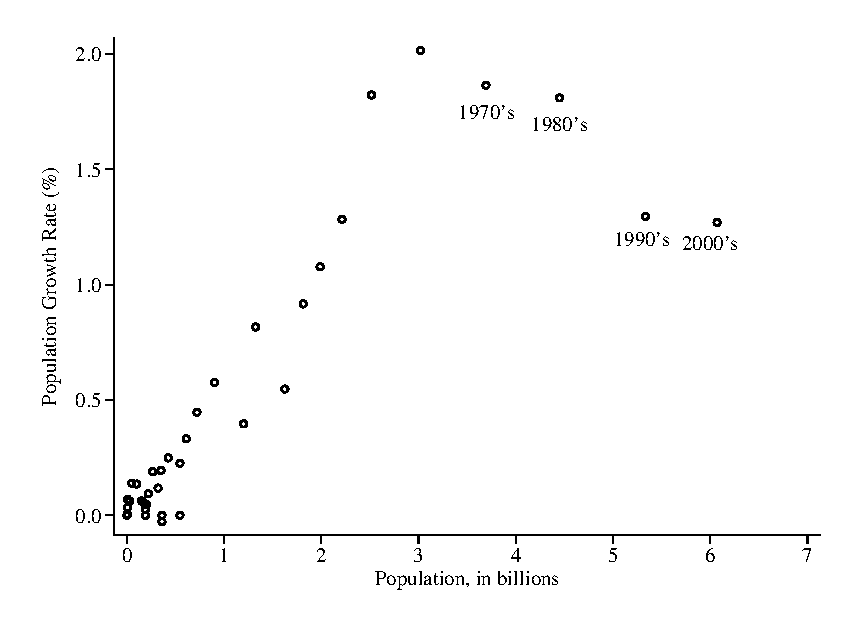
\includegraphics[width=1.0\textwidth]{figure_8_5.eps}
\end{center}
\vspace{-.5cm}\singlespacing {\footnotesize \textbf{Notes}: Replicates Figure 1 from Kremer (1992), with additional data on the 1990's and 2000's drawn from the UN Population Division. Growth rates are annualized.
}
\end{figure}

%%%%%% TABLES
\clearpage % start EACH table on its own page

\begin{table}[!htb]
\caption{OLS Regressions for Local School Taxes}\label{ivtable_B}
\par
\begin{center}
{\footnotesize
\begin{tabularx}{\textwidth}{lXXXXX}
\toprule
            & \multicolumn{5}{c}{Dep. variable is local school tax rev. per capita} \\
            &           &        &      & \multicolumn{2}{c}{By region:} \\ \cmidrule(lr){5-6}
            &           &        &      & North & South \\
            &     (1)   &    (2) & (3)  & (4) & (5)  \\            
           \midrule
Fraction 0-49 Acres ($\beta_1$)  &  2.002*  & 2.072** & 2.028** & 3.838** & -0.387 \\
             &  (1.072) & (1.053) & (0.994) & (1.883) & (0.245) \\ \\
Fraction 100-999 Acres ($\beta_2$) &  2.614** & 2.434** & 2.593** & 3.195** & -0.466 \\
             &  (1.128) & (1.027) & (1.320) & (1.543) & (0.363) \\ \\
Fraction 1000+ Acres ($\beta_3$)  &  -2.205  & -2.328 & -0.840   & 1.790   & -1.149 \\
             &  (2.254) & (2.349) & (3.534) & (16.006)& (0.875)  \\ \\
Log real estate value (p.c) &  0.525***& 0.220  & 0.224    & 0.011   & 0.120 \\
                   &  (0.174) & (0.154)& (0.150)  & (0.307) & (0.095) \\ \\
Log assessed value (p.c.) &          & 0.569**& 0.568**  & 1.253** & 0.156** \\
                   &          & (0.268)& (0.266)  & (0.521) & (0.076) \\ \\
Log avg. farm size &         &        & -0.133   & 0.476   & 0.020 \\
                   &          &        & (0.439)  & (0.930) & (0.105) \\ \\
R-squared          &  0.79 & 0.80 & 0.80 & 0.67& 0.82  \\
Observations       &  1345     & 1345     & 1345    & 596 & 749 \\
States             &  33     & 33     &  33    & 19  & 14  \\
\bottomrule
\end{tabularx}
}
\end{center}
\singlespacing {\footnotesize {\it Notes:}  Standard errors, clustered at the state level, are reported in parentheses. * denotes significance at 10\%, ** denotes 5\%, and *** denotes 1\%. The excluded category of farm sizes is 50-99 acres. All regressions include state fixed effects, and controls for log output per capita, the percent of black population, the percent of children in the population, and the log of population size.}
\end{table}

\clearpage

\begin{table}[!htb]
\begin{center}
\caption{Estimates of Malthusian Tightness, $\beta$, by Crop Suitability, 2000CE}
\label{TAB_beta_crops}
{\footnotesize
\begin{tabularx}{\textwidth}{lXXXXXX}
\toprule
\multicolumn{7}{l}{Dependent Variable in all panels: Log caloric yield ($A_{isc}$)} \\ \\
\multicolumn{7}{l}{Panel A: Samples defined by crop family (wheat vs. rice):} \\ \\
 & \multicolumn{2}{c}{By suitability:} & \multicolumn{2}{c}{By max calories:} & \multicolumn{2}{c}{By harvest area:}\\ \cmidrule(lr){2-3} \cmidrule(lr){4-5} \cmidrule(lr){6-7} 
 & Wheat & Rice & Wheat  & Rice  & Wheat  & Rice \\
 & Only & Only &  $>33\%$ & $>33\%$ & $>50\%$ & $>50\%$   \\
 & (1) & (2) & (3) & (4) & (5) & (6) \\
\midrule
Log rural density   &       0.228&       0.132&       0.191&       0.112&       0.205&       0.133\\
                    &     (0.021)&     (0.018)&     (0.016)&     (0.017)&     (0.015)&     (0.012)\\
\midrule
p-value $\beta=0$   &       0.000&       0.000&       0.000&       0.000&       0.000&       0.000\\
p-value $\beta=\beta^{Wheat}$&            &       0.000&            &       0.001&            &       0.000\\
Countries           &          91&          81&          83&          71&          74&          84\\
Observations        &       10661&        9088&       10786&        8217&       10708&        7564\\
Adjusted R-square   &        0.24&        0.20&        0.21&        0.18&        0.20&        0.18\\

\midrule
\\
\multicolumn{7}{l}{Panel B: Samples with other restrictions (using suitability to distinguish crop families)} \\ \\
 & \multicolumn{2}{c}{Urban Pop. $<25K$:} & \multicolumn{2}{c}{Ex. Europe/N. Amer.:} & \multicolumn{2}{c}{Rural dens. $>$ 25th P'tile:}\\ \cmidrule(lr){2-3} \cmidrule(lr){4-5} \cmidrule(lr){6-7}
  & Wheat Only& Rice Only & Wheat Only& Rice Only& Wheat Only& Rice Only\\
 & (1) & (2) & (3) & (4) & (5) & (6) \\
\midrule
Log rural density   &       0.261&       0.143&       0.242&       0.133&       0.281&       0.185\\
                    &     (0.022)&     (0.021)&     (0.033)&     (0.018)&     (0.035)&     (0.019)\\
\midrule
p-value $\beta=0$   &       0.000&       0.000&       0.000&       0.000&       0.000&       0.000\\
p-value $\beta=\beta^{Wheat}$&            &       0.000&            &       0.003&            &       0.015\\
Countries           &          83&          75&          24&          70&          89&          77\\
Observations        &        7648&        6662&         824&        8826&        7237&        7082\\
Adjusted R-square   &        0.29&        0.24&        0.19&        0.14&        0.27&        0.22\\

\bottomrule
\end{tabularx}
}
\end{center}
\vspace{-.5cm}\singlespacing {\footnotesize \textbf{Notes}: Conley standard errors, adjusted for spatial auto-correlation with a cutoff distance of 500km, are shown in parentheses. All regressions include province fixed effects, a constant, and controls for the district urbanization rate and log density of district nighttime lights. The coefficient estimate on rural population density indicates the value of $\beta$, see equation (\ref{EQ_ref}). Rural population is from HYDE database \citep{barro2016}, and caloric yield is the author's calculations based on the data from \citet{ajs2016}. Inclusion of districts in the regression is based on the listed criteria related to crop families. See text for all crops included in the wheat and rice families, and for details of the inclusion criteria.
}
\end{table}
\end{document}
